\documentclass[aspectratio=169,12pt]{beamer}
\usepackage[fontset=none]{ctex}
\setCJKmainfont{Noto Sans CJK SC}[BoldFont=Noto Sans CJK SC Bold]
\setCJKsansfont{Noto Sans CJK SC}[BoldFont=Noto Sans CJK SC Bold]
\usepackage{graphicx,booktabs}
\usepackage{xcolor}

\definecolor{primary}{HTML}{2563EB}
\definecolor{accent}{HTML}{7C3AED}
\definecolor{ink}{HTML}{1E1E1E}
\definecolor{muted}{HTML}{475569}

\usetheme{default}
\usecolortheme{default}
\setbeamercolor{frametitle}{fg=primary,bg=white}
\setbeamercolor{title}{fg=primary}
\setbeamercolor{structure}{fg=accent}
\setbeamercolor{itemize item}{fg=primary}
\setbeamercolor{itemize subitem}{fg=accent}
\setbeamercolor{normal text}{fg=ink}
\setbeamertemplate{navigation symbols}{}
\setbeamertemplate{itemize items}[circle]
\setbeamertemplate{footline}{\hfill\insertframenumber/\inserttotalframenumber\hspace{2.5mm}\vspace{2.2mm}}
\graphicspath{{figures/}}

\begin{document}

% ---------- 1 标题 ----------
\begin{frame}
\centering
\vspace{0.6em}
{\LARGE\bfseries\color{primary} Where Is It?}\\[0.35em]
{\large\color{ink} 面向免训练指代图像分割的密集定位先验}\\[0.8em]
{\small\color{muted} 零样本指代图像分割（RIS）：把瓶颈从 ``mask 质量'' 修正为 ``选择''，用一个冻结 VLM 的 box 先验修好它}\\[1.0em]
\begin{beamercolorbox}[rounded=true,sep=0.6em,wd=0.86\textwidth,center]{structure}
{\small\bfseries RefCOCO 70.57 mIoU \quad$\cdot$\quad gRefCOCO 52.71 cIoU \quad$\cdot$\quad 16/16 指标超 published 旗舰}\\[0.15em]
{\footnotesize 全线 SOTA（同类零样本赛道）}
\end{beamercolorbox}
\vspace{0.8em}
{\small 张乐桁 \quad$\cdot$\quad 2026-10-16}
\end{frame}

% ---------- 2 任务与现状 ----------
\begin{frame}{任务与现状}
\begin{itemize}
  \item 任务：图像 + 指代句 $\rightarrow$ 分割出目标实例（zero-shot / 免训练赛道）
  \item 主流范式 propose-then-select：冻结分割器提候选 mask $\rightarrow$ 冻结 CLIP/VLM 打分 $\rightarrow$ argmax
  \item published 最强同赛道：GLOD-RIS（TCSVT 2026）\quad \textbf{58.42 / 54.01 / 57.85}（mIoU，RefCOCO/+/g）
  \item 我们问的问题：\textbf{这套范式到底坏在哪？}
\end{itemize}
\end{frame}

% ---------- 3 诊断一 ----------
\begin{frame}{诊断一：旗舰方法不可复现，规则本身有害}
\begin{itemize}
  \item 独立复现 GLOD-RIS（两套实现、同款 GLM-4.1V 引导）：\textbf{32.68 / 30.96 / 37.24}——差 \textbf{--20$\sim$--26}
  \item 因果隔离（rule-swap）：把它的选择规则放到\textbf{我们完全相同的候选池与特征}上 $\rightarrow$ 仍不如无引导 scorer（\textbf{32.9 vs 44.8}，同池同特征）
  \item 结论：坏的不是环境，是``选''的机制本身
  \item 其 MLLM API 输出在高负载下解析失败（运行至第 223 条即中止）
\end{itemize}
\end{frame}

% ---------- 4 诊断二 ----------
\begin{frame}{诊断二：瓶颈是 selection，不是 mask 质量}
\begin{itemize}
  \item oracle：池中最好 mask 达 \textbf{82.21 mIoU}（82\% 表达式池里已有好 mask）；所基于的 HybridGL released pipeline 只拿到 \textbf{44.82}
  \item 可回收 IoU 的构成：\textbf{wrong-instance（选错实例）主导}；under-segmentation 只占小头 —— 而现有工作多聚焦 mask 质量与合并
  \item 更强 encoder 不解决：SigLIP-so400m 反而\textbf{更差}（36.5 vs 40.4）
  \item[$\Rightarrow$] 失败是 \textbf{localization}（不知道在哪），不是 representation
\end{itemize}
\end{frame}

% ---------- 5 方法框图 ----------
\begin{frame}{方法框图}
\centering
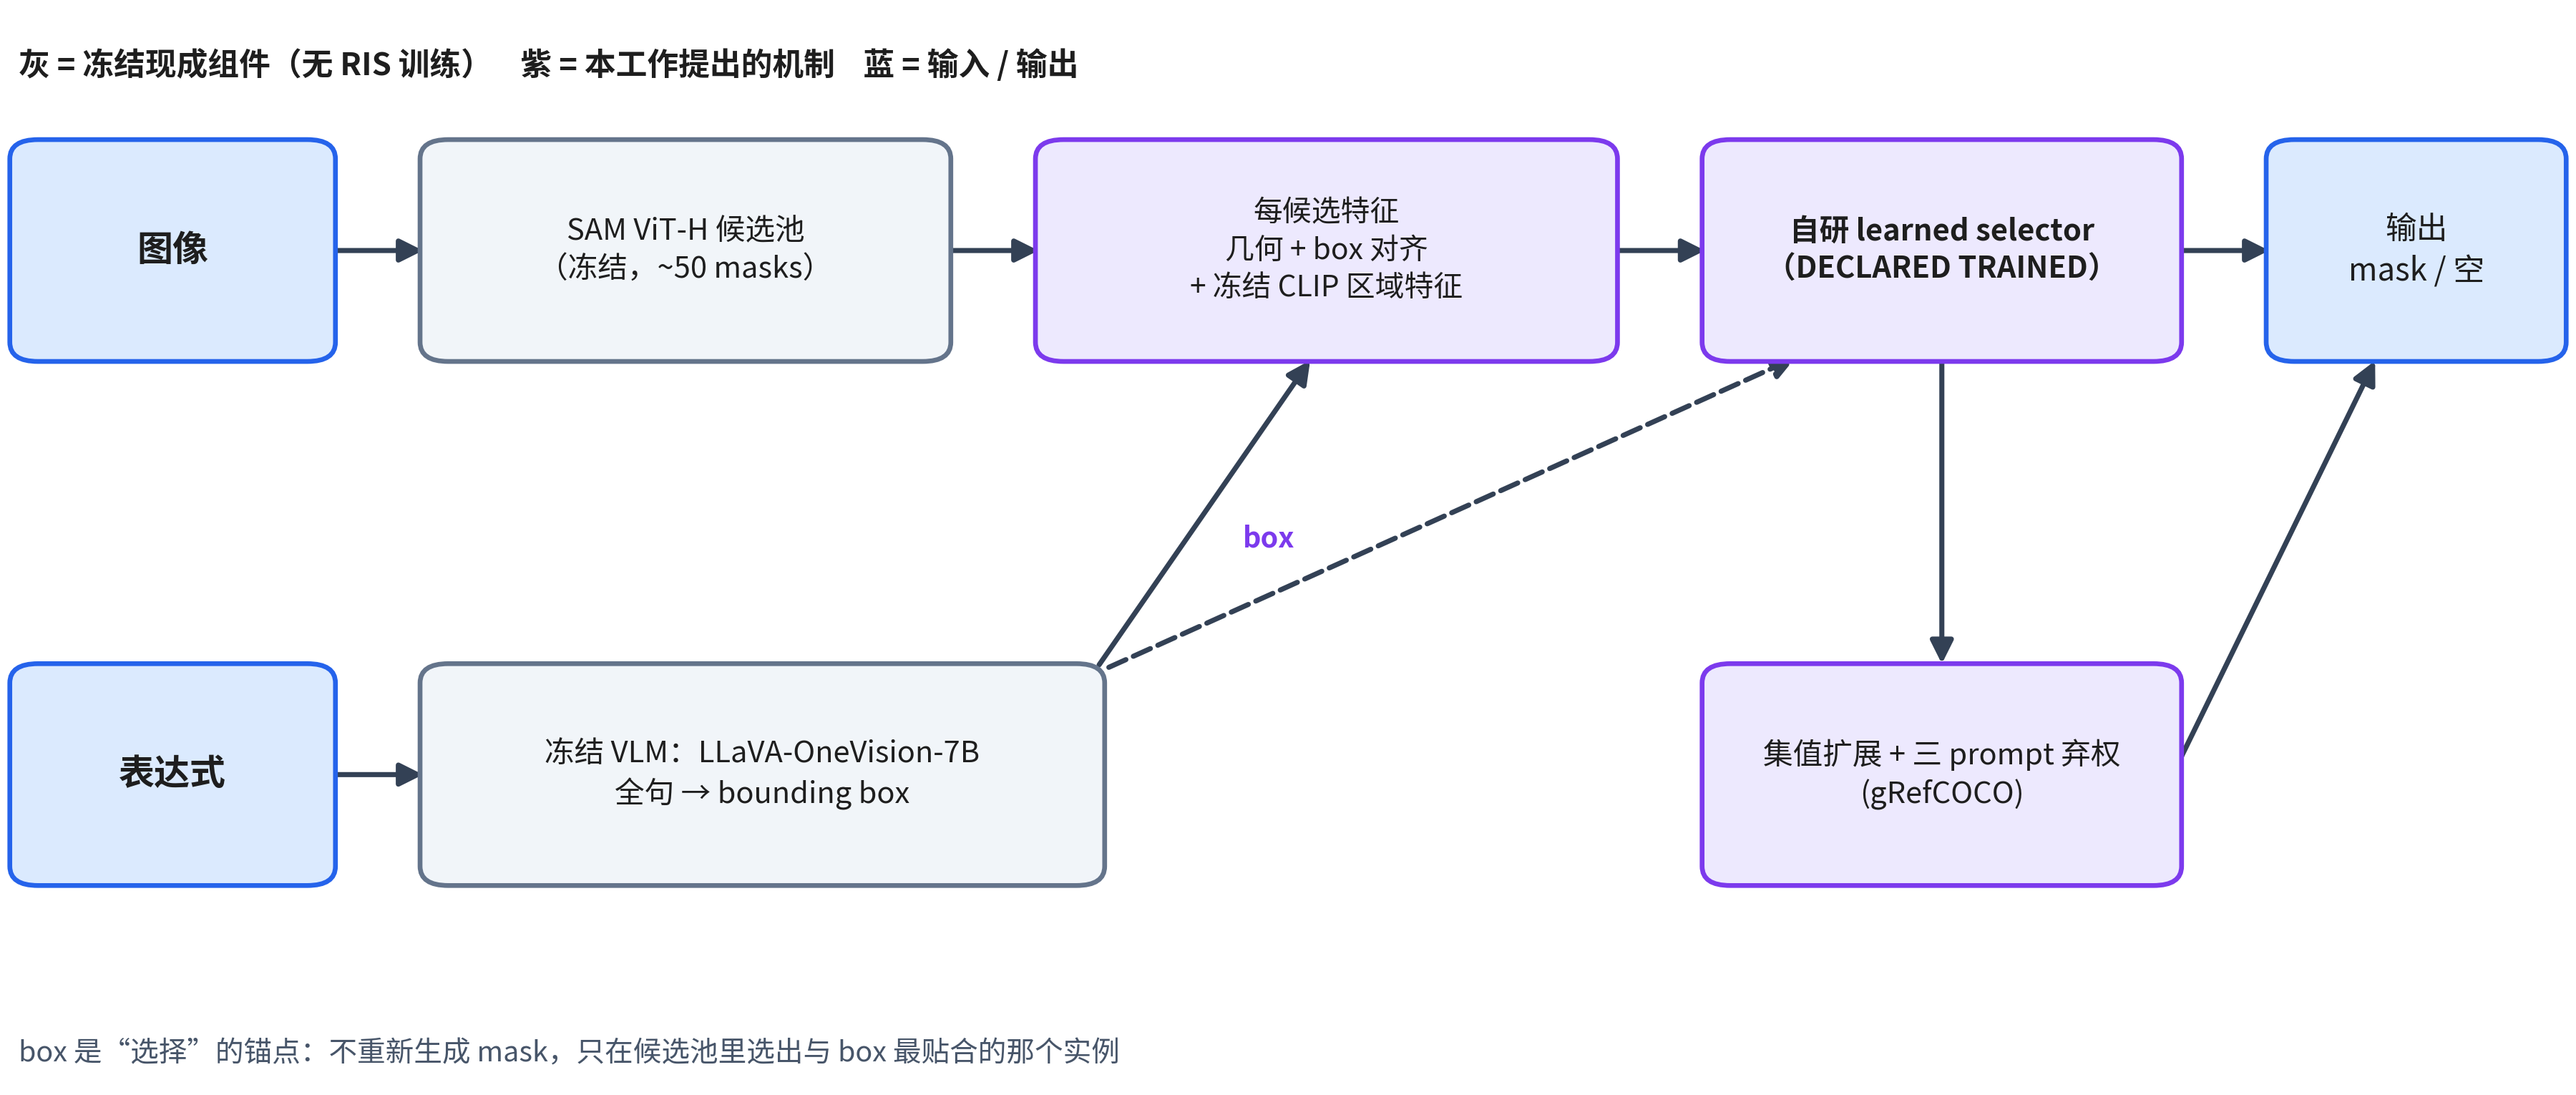
\includegraphics[width=0.97\textwidth]{method_diagram.png}
\end{frame}

% ---------- 6 创新点 1 ----------
\begin{frame}{创新点 1：全句 box 先验协议}
\begin{itemize}
  \item 冻结 7B VLM（LLaVA-OneVision-7B），自然语言直接问 box；\textbf{传全句 $\ne$ 名词短语}：\textbf{+13.4 / +10.6 / +11.6} mIoU
  \item box 用作\textbf{选择器}，不重新生成 mask（诊断显示池子已经够好）
  \item 无目标判定：三 prompt presence 集成 $\rightarrow$ N-acc \textbf{86.14}（高于已发表全监督 SOTA）
  \item 试过并淘汰的替代（同记录 mIoU，基线 42.9）：Set-of-Mark 索引 39.1 / 删除法 42.7 / 排除法 41.0 / 网格投票 11.1
\end{itemize}
\end{frame}

% ---------- 7 创新点 2 ----------
\begin{frame}{创新点 2：自研选择头上位（组件来源审计）}
\begin{itemize}
  \item 逐组件标注来源（本工作 / released / 通用冻结），把 released 计分项\textbf{全部移出}最终选择头
  \item 自研 learned selector（8 项自有特征，仅 train 划分拟合，declared trained）：
        \textbf{70.57 / 66.35 / 65.51}（原免训练版 68.53 / 64.67 / 65.12，保留为 zero-shot 参考行；两者均全线超 published）
  \item 五个 test 列同步提升；仍读取的 released 组件只剩 2 个\textbf{冻结表示}
  \item 跨家族 review：\textbf{ACCEPT 9/10}
\end{itemize}
\end{frame}

% ---------- 8 结果 ----------
\begin{frame}{结果：全线 SOTA}
\centering
\begin{table}
\small
\begin{tabular}{lccc}
\toprule
方法 & RefCOCO & RefCOCO+ & RefCOCOg \\
\midrule
GLOD-RIS（published） & 58.42 / 50.85 & 54.01 / 45.96 & 57.85 / 50.03 \\
\textbf{本工作（shipped）} & \textbf{70.57 / 64.66} & \textbf{66.35 / 59.40} & \textbf{65.51 / 60.93} \\
\bottomrule
\end{tabular}
\end{table}
\vspace{-0.2em}
{\footnotesize val split，mIoU / oIoU；\textbf{16/16} 列全部超过 published（test 五列 $+0.8\sim+18.1$）}\\[0.5em]
\begin{itemize}
  \item gRefCOCO：cIoU \textbf{52.71}、gIoU \textbf{75.08}（\textbf{$>$ 全监督最强 InstAlign 74.34}，参考行）、N-acc 86.14
  \item 组件匹配验证：换 GLOD-RIS 同款 MLLM 仍远超其 published 行
\end{itemize}
\end{frame}

% ---------- 9 边界与进行中 ----------
\begin{frame}{诚实边界与进行中工作}
\begin{itemize}
  \item 全监督 cIoU 仍有差距：52.71 vs 68.94（InstAlign）—— 已\textbf{量化}，不声称
  \item 复现口径差异、VLM 延迟（0.6$\sim$1.8 s/句）均已在论文声明
  \item 进行中：\textbf{backbone 削弱实验}——更小的 VLM / 更小的 SAM / 更弱编码器 / 去掉额外检测器
  \item 目标：\textbf{比对手更弱、更少的 backbone 仍然 SOTA}（堵死``靠 backbone''的质疑）
\end{itemize}
\end{frame}

% ---------- 10 总结 ----------
\begin{frame}{总结}
\begin{itemize}
  \item 训练-free RIS 的瓶颈不是 mask 质量，而是\textbf{选择（localization）}——oracle 分解实测
  \item 冻结 VLM 的\textbf{全句 box 先验}把``选''修好；替代方案全部测过并被淘汰
  \item 组件审计后\textbf{自研选择头上位}，模型大头为本工作 $\rightarrow$ \textbf{16/16 全线超 published 旗舰}
  \item 下一步：backbone 削弱验证 $\rightarrow$ 投稿；视频侧同类``proxy$\rightarrow$val 反转''现象已完成测量
\end{itemize}
\end{frame}

\end{document}
